\documentclass[8pt]{extarticle}
\usepackage[a4paper,headsep=10pt, top=30pt, bottom=30pt, left=30pt, right=30pt, footskip=10pt]{geometry}
\usepackage{listings}	
\usepackage{setspace}			%used for \begin{spacing}\end{spacing}-> vertical space setting
\usepackage{amsfonts} 			%used for \mathbb{} -> numerical sets
\usepackage{amsmath}			%used for \text{} inside math equations
\usepackage{enumitem}
\usepackage{bm}					%used for bold math expressions
\usepackage{calc}				%used for algebric operations inside \newenvironment
\usepackage{fancyhdr}			%used for head and foot settings
%\usepackage{draftwatermark}		%used for watermark
\usepackage{clrscode3e}		%pseudocde 
\usepackage{graphics}



%%watermark settings
%\SetWatermarkText{Vici Francesco}
%\SetWatermarkScale{2}
%\SetWatermarkAngle{60}
%%end watermark settings



\fancypagestyle{plain}
{
\fancyhead{}\fancyfoot{}
\fancyhead[C]{\vspace{0pt}   Sommario Algortmi e Strutture Dati}
\fancyfoot[R]{Vici Francesco}
\fancyfoot[C]{\thepage}
}
\pagestyle{plain}



\newenvironment{formulario}
{
\setlength{\columnsep}{3em}
\twocolumn
\lstset{tabsize=3}
\begin{spacing}{1}
\begin{flushleft}
}{
\end{flushleft}
\end{spacing}
}



\newenvironment{tcenter}{
  \par
  \centering
  \setlength{\parskip}{0pt} % Rimuovi spaziatura verticale
  \noindent
}{
  \par
}



\newenvironment{Descr}
{
	\begin{description}[topsep=0pt,itemsep=0pt,partopsep=0pt, parsep=0pt]
}{
	\end{description}
}



\newenvironment{descr}[1]
{
\setlist[description,1]{leftmargin=2em + (2em * #1),labelindent=0em + (2em * #1)}
\begin{description}[topsep=0pt,itemsep=0pt,partopsep=0pt, parsep=0pt]
}{
\end{description}
}



\newenvironment{code}[1]
{
\begin{codebox}
\Procname{$#1$}
}{
\end{codebox}
}



\newenvironment{myParagraph}[1]
{
\begin{tcenter}
\textbf{#1}
\end{tcenter}
}{
\myRule
}



\newcommand{\myRule}{\rule{250pt}{0.1pt}}
\newcommand{\bo}[1]{\textbf{#1}}
\newcommand{\co}[1]{\textit{#1}}
\newcommand{\R}{\mathbb{R}}
\newcommand{\N}{\mathbb{N}}
\newcommand{\la}{\leftarrow}
\newcommand{\ra}{\rightarrow}
\newcommand{\sse}{\leftrightarrow}
\newcommand{\floor}[1]{\lfloor #1 \rfloor}
\newcommand{\modulo}[1]{\left\vert #1 \right\vert}

\newcommand{\FOR}[1]{\For $#1$ \Do}
\newcommand{\WHILE}[1]{\While $#1$ \Do}
\newcommand{\IF}[1]{\If $#1$ \Then}
\newcommand{\ELSEIF}[1]{\ElseIf $#1$\Then}
\newcommand{\ELSE}{\Else}
\newcommand{\COMMENT}{\qquad\Comment}
\newcommand{\RETURN}{\Return}
\newcommand{\END}{\End}





\begin{document}
	\begin{formulario}

%PARAGRAFO 1
		\begin{tcenter}
\textbf{ALGORITMO}
		\end{tcenter}
Un algoritmo è una sequenza finita di operazioni, anche dette istruzioni, che riceve un input e restituisce un output al fine di risolvere un determinato problema.\\
\myRule

%PARAGRAFO 2
		\begin{tcenter}
\textbf{PROBLEMA DELL'ORDINAMENTO} 
		\end{tcenter}
Data in input una sequenza di numeri $n$ numeri $<a_1,a_2,...,a_n>$ si vuole ottenere in output una permutazione tale che:
		\begin{tcenter}
$<a_{1}^{'},a_{2}^{'},...,a_{n}^{'}>$ con $a_{1}^{'} \leq a_{2}^{'} \leq ... \leq a_{n}^{'} $
		\end{tcenter}
Il tipo di algoritmo usato per l'ordinamento dipende da fattori come: numero di elementi, ordinamento iniziale, tipo di memorizzazione usata, ecc...\\
\myRule

%PARAGRAFO 3
		\begin{tcenter}
\textbf{CORRETTEZZA DI UN ALGORITMO}
		\end{tcenter}
Un algoritmo viene detto "corretto" se ad ogni istanza di input termina con l'output giusto.\\
\textbf{Induzione Matematica}: Supponendo di voler dimostrare che la proprietà $P(n)$ vale per qualsiasi $n\in \mathbb{N}$. Definisco l'insieme universo $U={n\in\mathbb{N}\text{ t.c. vale } P(n)}$. Allora:\\

	\begin{descr}{1}
		\item[Passo Base]$\rightarrow$ dimostro che vale $P(1)$ o $P(0)$; 
		\item[Passo Induttivo]$\rightarrow$ suppongo che $P(n)$ valga per un generico $n$. Posso dunque concludere che $U$ coincide con $\mathbb{N}$.
	\end{descr}
\textbf{Invariante di Ciclo}: formulo un'affermazione che deve essere verificata in 3 diversi momenti:\\
	\begin{descr}{1}
		\item[Inizializzazione]$\rightarrow$ l'I.C. deve essere vera prima della prima iterazione del ciclo;
		\item[Conservazione]$\rightarrow$ l'I.C. deve essere vera prima della successiva iterazione del ciclo;
		\item[Conclusione]$\rightarrow$ l'I.C. al termine del ciclo deve fornire una condizione che permetta di verificare se l'output dell'algoritmo è corretto.
	\end{descr}
\myRule

%PARAGRAFO 4
	\begin{tcenter}
\textbf{ANALISI ASINTOTICA}
	\end{tcenter}
Il calcolo asintotico è usato per analizzare la complessità di un algoritmo ovvero per stimare quanto tale complessità aumenta all’aumentare della dimensione dell’input. Uso la funzione $T(n)$ in quanto la risorsa considerata è il tempo (misurato in operazioni elementari). Allora:
	\begin{descr}{0}
	
\item[Notazione $\bm{O}$] $\rightarrow$ $g(n)$ è un limite asintotico superiore per $f(n)$ ed è definito come:
		\begin{tcenter}
$\bm{O(g(n))} =\{ f(n): \; \exists \, c\in\R^+ ,n_0\in\N $ t.c. $ \bm{0\leq f(n)\leq c\cdot g(n)} \;\; \forall\, n\geq n_0 \}$
		\end{tcenter} 
		
\item[Notazione $\bm{o}$] $\rightarrow$ è definito come:
		\begin{tcenter}
$\bm{o(g(n))} =\{ f(n): \; \forall \, c\in\R ,\,\exists n_0>0\in\N $ t.c. $ \bm{0\leq f(n)< c\cdot g(n)} \;\; \forall\, n\geq n_0 \}$
		\end{tcenter} 
		
\item[Notazione $\bm{\Omega}$] $\rightarrow$ $g(n)$ è un limite asintotico inferiore per $f(n)$ ed è definito come:
		\begin{tcenter}
$\bm{\Omega(g(n))} =\{ f(n): \; \exists \, c\in\R^+ ,n_0\in\N $ t.c. $ \bm{0\leq c\cdot g(n)\leq f(n)} \;\; \forall\, n\geq n_0 \}$
		\end{tcenter} 		
		
\item[Notazione $\bm{\omega}$] $\rightarrow$ è definito come:
		\begin{tcenter}
$\bm{\omega(g(n))} =\{ f(n): \; \forall \, c\in\R ,\,\exists n_0>0\in\N $ t.c. $ \bm{0\leq c\cdot g(n)< f(n)} \;\; \forall\, n\geq n_0 \}$
		\end{tcenter}

\item[Notazione $\bm{\Theta}$] $\rightarrow$ $g(n)$ è un limite asintoticamente stretto per $f(n)$ ed è definito come:
		\begin{tcenter}
$\bm{\Theta(g(n))} =\{ f(n): \; \exists \, c_1,c_2\in\R^+ ,n_0\in\N $ t.c. $ \bm{0\leq c_1\cdot g(n)\leq f(n)\leq c_2\cdot g(n)} \;\; \forall\, n\geq n_0 \}$
		\end{tcenter} 
	\end{descr}
	
	\begin{descr}{1}
		\item[Teorema]: $f(n)=\Theta g(n) \text{ SSE } f(n)=O g(n) \text{ e } f(n)=\Omega g(n)$
		\item[Proprietà]: 
		\begin{descr}{0}
			\item[Transitiva]: $f(n)=\Theta(g(n))\text{ e }g(n)=\Theta(h(n)) \implies f(n)=\Theta(h(n))$ \quad (vale anche per $O,o,\Omega,\omega$);
			\item[Riflessiva]: $f(n)=\Theta(f(n))$ \quad (vale anche per $O,\Omega$);
			\item[Simmetria]: $f(n)=\Theta(g(n))\Leftrightarrow g(n)=\Theta(f(n))$;
			\item[Simmetria Trasposta]: $f(n)=O(g(n))\Leftrightarrow g(n)=\Omega(f(n))$ $f(n)=o(g(n))\Leftrightarrow g(n)=\omega(f(n))$
		\end{descr}
	\end{descr}
\myRule
%PARAGRAFO 5
	\begin{tcenter}
\textbf{CLASSI DI COMPLESSITA'}
	\end{tcenter}
Per categorizzare la complessità degli algoritmi faccio riferimento alla crescita di funzioni semplici. Le classi sono:\\
	\begin{descr}{0}
	\item[$\bm{O(1)}$] $\rightarrow$ complessità costante;
	\item[$\bm{O(kn)}$] con $k<1 \rightarrow$ complessità sottolineare (\underline{ES}: ricerca sequenziale);
	\item[$\bm{O(n)}$] $\rightarrow$ complessità lineare (\underline{ES}:ricerca sequenziale);
	\item[$\bm{O(n\cdot \ln n)}$] $\rightarrow$ (\underline{ES}: algoritmi di ordinamento ottimi);
	\item[$\bm{O(n^k)}$] con $k\geq 2\rightarrow$ (\underline{ES}: BubbleSort con $O(n^2)$); 
	\item[$\bm{O(k^n)}$] $\rightarrow$ complessità esponenziale;
	\end{descr}
\myRule

%PARAGRAFO 6
	\begin{tcenter}
\textbf{ALGORITMI ITERATIVI - INSERTION SORT}
	\end{tcenter}
È uno degli algoritmi iterativi più semplici. Ordina "in place" ed è efficiente per insiemi quasi ordinati. Lo pseudocodice è:
		\begin{codebox}
\Procname{$\proc{Insertion-Sort}(A)$}
\li \For $j \la 2$ \To $\attrib{A}{length}$ \Do
	\li $\id{key} \la A[j]$
	\li $i \la j-1$
	\li \While $i > 0$ \const{and} $A[i] > \id{key}$ \Do
		\li $A[i+1] \la A[i]$
		\li $i \la i-1$
	\End
	\li $A[i+1] \la \id{key}$
\End
		\end{codebox}
\textbf{Correttezza con I.C.} \\
"All'inizio di ogni iterazione del ciclo \textit{for}, il sottoarray $A[1,\dots,j-1]$ è ordinato ed è formato dagli stessi elementi che erano originariamente in $A[1,\dots,j-1]$, ma ordinati".\\
\textbf{Costo}
		\begin{descr}{1}
\item[Caso Ottimo] (Array Ordinato): $O(n)\rightarrow$ non si entra mai nel \textit{while} ma si esegue ogni volta il confronto, al contrario si esegue sempre il \textit{for}.
\item[Caso Peggiore] (Array Ordinato al Contrario): $O(n^2)\rightarrow$ si esegue il \textit{while} per il numero massimo di volte, il costo del \textit{for} è irrilevante rispetto a quello del \textit{while}.
\item[Caso Medio] (Array Disordinato): $O(n^2)\rightarrow$ il costo dipende dall'ordine ma statisticamente il \textit{while} verrà eseguito soltanto la metà delle volte rispetto al caso peggiore, il costo rimane quadratico. 
		\end{descr}
\myRule

%PARAGRAFO 7
		\begin{tcenter}
\textbf{ALGORITMI ITERATIVI - SELECTION SORT}
		\end{tcenter}
È un algoritmo molto semplice, opera "in place". Il suo obbiettivo è quello di trovare il minimo all'interno dell'array e inserirlo nella sequenza ordinata fino a qual momento. Lo pseudocodice è: \\		
		\begin{code}{SelectionSort(A)}
\li $n\la\attrib{A}{lenght}$
\li \For $j\la1 \To n-1$ \Do
	\li $\id{smallest}\la j$
	\li \For $i \la j+1 \To n$ \Do
		\li \If $A[i]<A[\id{smallest}]$ \Then
			\li $\id{smallest}\la i$
		\End
	\End
	\li \bf{exchange }$A[j]\sse A[smallest]$
		\end{code}				
\textbf{Correttezza con I.C.}
		\begin{descr}{1}
\item[Ciclo Interno] $\rightarrow$ "All'inizio della $i$-esima iterazione del \textit{for} interno, $A[min]$ è minore o uguale di ogni elemento di $A[j,\dots,i-1]$ cioè $\forall j\in [j,\dots,i-1]$ si ha che $A[min]\leq A[j]$". 
\item[Ciclo Esterno] $\rightarrow$ "All'inizio di ogni iterazione del ciclo \textit{for} esterno, il sottoarray $A[1,\dots,j-1]$ è ordinatoe composto solo dagli elementi più piccoli dell'array $A$".
		\end{descr}
\bo{Costo}\\
In questo caso è sempre $O(n^2)$ perché, sia nel caso migliore sia nel caso peggiore, i due cicli \co{for} vengono comunque eseguiti. L'unica riga che può non essere eseguita è la 6, che è trascurabile al fine del calcolo del costo.\\
\myRule

%PARAGRAFO 8
		\begin{tcenter}
\bo{COMPLESSITÀ ALGORITMI RICORSIVI}
		\end{tcenter}
\bo{Equazione di Ricorrenza}\\
Si usa per stimare il tempo di esecuzione di algoritmi ricorsivi. Si fa rifermento alla divisione e combinazione di vari sottoproblemi. Infatti l'equazione è:
		\begin{tcenter}
$\mathbf{T(n)=		
		\begin{cases}
\Theta(1) \qquad \text{se } n\leq c\\
aT(\frac{n}{b})+D(n)+C(n) \qquad \text{altrimenti}
		\end{cases}}$
		\end{tcenter}  
Se $n\leq c$ con $c$ una costante, si ha il caso base; altrimenti si divide in $a$ sottoproblemi di dimensione $\frac{1}{b}$. Questo implica un costo $D(n)$ di divisione del problema e un costo $C(n)$ di combinazione dei sottoproblemi. I metodi di risoluzione di tale equazione sono:
		\begin{descr}{1} 
\item[Metodo di Sostituzione] $\rightarrow$ Ipotizzo una soluzione e la dimostro con un'induzione matematica:\\
			\begin{descr}{0}
\item[1.] indovino una soluzione e formulo un'ipotesi induttiva;
\item[2.] sostituisco nell'equazione di ricorrenza le epressioni $T(\cdot)$;
\item[3.] dimostro che è valida anche per il caso base.
			\end{descr}
La soluzione per una ricorrenza può essere:
			\begin{descr}{0}
\item[Esatta] $\rightarrow$ se la ricorrenza è formata da una funzione esatta allora anche la soluzione sarà sempre esatta;
\item[Asintotica] $\rightarrow$ mi riconduco ad una soluzione esatta, ipotizzo per prima cosa che la soluzione $T(n)$ sia per esempio un $O$ di qualche funzione e poi cerco le costanti che verificano l'ipotesi induttiva (quelle presenti nella definizione di $O$). 
			\end{descr}
\item[Metodo dell'Albero di Ricorsione] $\rightarrow$ È un metodo grafico per arrivare alla soluzione. L'albero deve sempre condurre ad un'equazione esatta. I nodi rappresentano i costi dei vari sottoproblemi e permette di aver un'idea del costo complessivo di tutte le esecuzioni dell'algoritmo. Si sommano i costi di tutti i vari sottolivelli per poi fare una somma complessiva di tali sottolivelli.
\item[Metodo dell'Esperto] $\rightarrow$ Sia $T(n)$ una funzione definita sui naturali dalla ricorrenza $T(n)=aT(\frac{n}{b})+f(n)$ con $a\geq 1, b>1$ costanti e $f(n)>0$ asintoticamente, allora $T(n)$ può essere limitata nei seguenti modi:
			\begin{descr}{0}
\item[caso 1]$\rightarrow$ se $f(n)=O(n^{\log_b a-\epsilon})$ per qualche costante $\epsilon>0$ allora: 
				\begin{tcenter}
$\mathbf{T(n)=\Theta(n^{\log_b a})}$
				\end{tcenter} 
\item[caso 2]$\rightarrow$ se $f(n)=\Theta(n^{\log_b a})$ allora:
				\begin{tcenter}
$\mathbf{T(n)=\Theta(n^{\log_b a}\cdot \log_2 n)}$
				\end{tcenter}
\item[caso 3]$\rightarrow$ se $f(n)=\Omega(n^{log_b a+\epsilon})$ per qualche costante $\epsilon>0$ e $f(n)$ t.c. $a\;f(\frac{n}{b})\leq c\;f(n)$ per qualche costante $c<1$ e $\forall n\geq n_0$, allora:
				\begin{tcenter}
$\mathbf{T(n)=\Theta(f(n))}$
				\end{tcenter}
\item[Condizione di Regolarità:]
Devo assicurarmi che quando scendo nell'albero $f(\cdot)$ diventa più piccola.
			\end{descr}
\item[Albero di Ricorsione + Esperto]$\rightarrow$ Combinando i metodi precedentemente descritti ottengo:
			\begin{descr}{0}
\item[caso 1]$\rightarrow$ se il costo cresce dalla radice alle foglie ("Costo Dominato dalle Foglie"), allora:
				\begin{tcenter}
$\mathbf{T(n)=\Theta(n^{\log_b a})}$
				\end{tcenter}
\item[caso 2]$\rightarrow$ se il costo è circa lo stesso in ogni livello, allora:
				\begin{tcenter}
$\mathbf{T(n)=\Theta(n^{\log_b a}\cdot\log_2 n)}$
				\end{tcenter}
\item[caso 3]$\rightarrow$ se il costo decrementa dalla radice alle foglie ("Costo Dominato dalla Radice"), allora: 
				\begin{tcenter}
$\mathbf{T(n)=\Theta(f(n))}$
				\end{tcenter}
			\end{descr}
		\end{descr}
\myRule

%PARAGRAFO 9
		\begin{tcenter}
\bo{ALGORITMI RICORSIVI - MERGE SORT}
		\end{tcenter}
Divide ricorsivamente l'array da ordinare in due sottoarray di uguale lunghezza. Una volta arrivato alla lunghezza unitaria combina ricorsivamente i sottoarray ordinandoli. Lo pseudocodice è:
		\begin{code}{MergeSort(A,p,r)}
\li \IF{p<r} 
	\li $q\la \floor{(p+r)/2}$ 
	\li \proc{MergeSort}(A,p,q)
	\li \proc{MergeSort}(A,q+1,r)
	\li \proc{Merge}(A,p,q,r)
\End
		\end{code}		
		\begin{code}{Merge(A,p,q,r)}
\li $n_1 \la q-p+1$
\li $n_2 \la r-q$
\li \FOR{i \la 1 \To n-1} 
	\li $L[i] \la A[p+i-1]$
\End
\li \FOR{j \la 1 \To n_2} 
	\li $R[i] \la A[q+j]$
\End
\li $L[n_1+1]\la \infty$
\li $R[n_2+1]\la \infty$
\li $i \la 1$
\li $j \la 1$
\li \FOR{k \la p\To r}
	\li \IF{L[i]\leq R[j]}
		\li $A[k]\la L[i]$
		\li $i \la i+1$
	\li \Else
		\li $A[k]\la R[j]$
		\li $j \la j+1$
	\End
\End
		\end{code}		
\bo{Costo}\\
Ho che il costo di divisione è $D(n)=\Theta(1)$ mentre il costo di combinazione è $C(n)=\Theta(n)$ Inoltre ad ogni ricorrenza successiva l'algoritmo risolve $2$ problemi di dimensione $\frac{n}{2}$. Allora l'equazione di ricorrenza sarà: 
		\begin{tcenter}
$
T(n)=
		\begin{cases}
\Theta(1) \qquad\text{se }n=1 \\
2T(\frac{n}{2})+\Theta(1)+\Theta(n) \qquad\text{se }n>1
		\end{cases}
$
		\end{tcenter}
Poiché divido sempre il problema in 2 sottoproblemi di uguale dimensione è facile risolvere il problema con il metodo dell'albero di ricorrenza. Ogni livello ha costo $\Theta(n)$ ed essendo il numero di livelli $\log_2 n$ avrò che il costo del problema è:
		\begin{tcenter} 
$\mathbf{T(n)=}\Theta(n\cdot \log_2 n) + \Theta(n) + \Theta(1)=\mathbf{\Theta(n\cdot \log_2 n)}$
		\end{tcenter}
\myRule

%PARAGRAFO 10
		\begin{tcenter}
\bf{ALGORITMI RICORSIVI - QUICKSORT}
		\end{tcenter}
Divide ricorsivamente l'array da ordinare in due sottoarray grazie all'uso di due indici (ordina sul posto) grazie all'algoritmo "partition" per poi riordinarli e combinarli grazie all'algoritmo "quicksort". Lo pseudocodice è:

		\begin{code}{QuickSort(A,p,r)}
\li \IF{p<r}
	\li $q \la \proc{Partition}(A,p,r)$
	\li $\proc{QuickSort}(A,p,q-1)$
	\li $\proc{QuickSort}(A,q+1,r)$
\End
		\end{code}
		\begin{code}{Partition(A,p,r)}
\li $x\la A[r]$
\li $i\la p-1$
\li \FOR{j\la p \To r-1}
	\li \IF{A[j]\leq x}
		\li $i \la i+1$
		\li	 $\proc{Exchange }A[i] \sse A[j]$
	\End
\End
\li $\proc{Exchange } A[i+1]\sse A[r]$
\li \Return $i+1$	
		\end{code}
\bo{Costo}\\
		\begin{descr}{1}
\item[Partition] $\rightarrow$ ha costo fisso $\Theta(n)$.
\item[Quicksort] $\rightarrow$ il costo dipende dal partizionamento dei sottoarray. Infatti:
			\begin{descr}{0}
\item[Caso migliore] (sottoarray bilanciati) $\rightarrow$ ogni sottoarray ha dimensione $\leq \frac{n}{2}$ quindi il costo sarà $\Theta(\log_2 n)$;
\item[Caso peggiore] (sottoarray sbilanciati) $\rightarrow$ i due sottoarray sono di dimensione $0$ e $n-1$ quindi il costo complessivo sarà $\Theta(n^2)$;
\item[Caso Medio] $\rightarrow$ supponendo una suddivisione parzialmente sbilanciata (ad esempio 9 a 1) avremo un costo:
				\begin{tcenter}
$T(n)=T(\frac{9n}{10})+T(\frac{n}{10})+\Theta(n)=O(n\cdot \log_2 n)$
				\end{tcenter}
			\end{descr}
		\end{descr}
\myRule

%PARAGRAFO 11
	\begin{tcenter}
\bo{CENNI DI PROBABILITÀ}
	\end{tcenter}
Definisco $S$ come lo spazio degli eventi, ovvero come un insieme di eventi $E$ (esiti di esperimenti). Allora la probabilità $P$ che un evento si verifichi è:  
		\begin{tcenter}
		$\bm{P(E)=\frac{\text{casi favorevoli}}{\text{casi possibili}}}$
		\end{tcenter}
\bo{Proprietà:} 
	\begin{descr}{1}
\item[1.] $P(E)\geq 0 \quad \forall \text{ evento }E$;
\item[2.] $P(S)=1$;
\item[3.] $P(A \cup B)=P(A)+P(B)$ \quad se $A$ e $B$ sono mutuamente esclusivi;
\item[3.] $P(A \cup B)=P(A)+P(B)-P(A\cap B)$ \quad se $A$ e $B$ sono compatibili (cioè hanno eventi in comune).
	\end{descr}
\bo{Probabilità Composta:}
	\begin{descr}{1}
	
\item[Eventi Indipendenti]$\rightarrow$ Due eventi sono indipendenti se il realizzarsi di uno non influenza la probabilità di realizzarsi dell'altro. La probabilità che si realizzino entrambi è:
		\begin{tcenter}
$\bm{P(A\cap B)=P(A)\cdot P(B)}$
		\end{tcenter}
		
\item[Eventi Dipendenti]$\rightarrow$ Due eventi sono dipendenti se il realizzarsi di uno influenza la probabilità di realizzarsi dell'altro.  Indico con $P(B|A)$ la probabilità che si verifichi $B$ supponendo che si sia verificato $A$, allora la probabilità che si realizzino entrambi è:
		\begin{tcenter}
$\bm{P(A\cap B)= P(A)\cdot P(B|A)}$
		\end{tcenter}
		
	\end{descr}
\bo{Probabilità Condizionata:}
		\begin{tcenter}
$\bm{P(A|B)=\frac{P(A\cap B)}{P(B)}}$
		\end{tcenter}
		
		\begin{descr}{1}
\item[Teorema di Bayes] $\rightarrow$ Poiché $A\cap B=B\cap A$ ho che:
			\begin{tcenter}
$\bm{P(A\cap B)=P(B)P(A|B)=P(A)P(A|B)}$
			\end{tcenter}
		\end{descr}

	\begin{descr}{0}
\item[Variabile Aleatoria] $\rightarrow$ È l'insieme di tutti i possibili risultati che possono verificarsi in un esperimento.
\item[Distribuzione di Probabilità] $\rightarrow$ Elenca le probabilità di verificarsi di ogni valore della variabile aleatoria a cui si riferisce. La somma di tutte le probabilità di una distribuzione di probabilità è sempre pari a 1 (cioè $\sum P(X)=\sum_i P(x_i)=1$).
\item[Valore Atteso] $\rightarrow$ È il valore medio che mi aspetto da una lunga serie di osservazioni, ed è definito come: 
		\begin{tcenter}
$\bm{\mu=E[X]=\sum_{i=1}^n x_i\cdot P(x_i)}$
		\end{tcenter}
		\begin{descr}{0}
\item[Linearità]:
		\begin{tcenter}
$\bm{E[X+Y]=E[X]+E[Y]}$;\\
$g(x)=ax \implies \bm{E[aX]=aE[X]}$.
		\end{tcenter}
		\end{descr}
	\end{descr}
\myRule

%PARAGRAFO 12
		\begin{tcenter}
\bf{VARIABILI CASUALI INDICATRICI}
		\end{tcenter}
Dato uno spazio dei campioni $S$ e un evento $A$, si definisce variabile casuale indicatrice:
		\begin{tcenter}
$\bm{I\{A\}\text{ oppure }X_A=}		
		\begin{cases} 
1 \quad\text{se si verifica A;}\\
0 \quad\text{se non si verifica A}  
		\end{cases}$
		\end{tcenter}
		\begin{descr}{0}
\item[Lemma] $\rightarrow$ $E[X_a]=Pr\{ A \}$.
		\end{descr}
\myRule

%PARAGRAFO 13
		\begin{tcenter}
\bf{ALGORITMI RANDOMIZZATI}
		\end{tcenter}
Poiché non posso conoscere l'ordine in cui l'algoritmo riceverà gli input, non posso, allo stesso modo, conoscere la probabilità delle $n!$ possibili permutazioni. Uso l'algoritmo "random" per forzare l'ordine casuale. Lo pseudocodice è:
		\begin{code}{RandomizeInPlace(A)}
\li $n \la A.lenght$
\li \FOR{i \la 1 \To n}
	\li $\proc{excange } A[i]\sse A[\proc{Random}(i,n)]$
\End
		\end{code}
\bo{Costo:}\\
$\Theta(1)$ per ogni iterazione, quindi $\Theta(n)$ in totale.
\myRule

%PARAGRAFO 14
		\begin{tcenter}
\bo{ALGORITMI RANDOMIZZATI - QUICKSORT} 
		\end{tcenter}
Cerco di avvicinarmi il più possibile all'ipotesi di caso medio. Per farlo, randomizzo la scelta del pivot $q$ per l'algoritmo "partition", mentre l'algoritmo "quicksort" rimane uguale. Lo pseudocodice è: 
		\begin{code}{RandomizedPartition(A,p,r)}
\li $i\la \proc{Random}(p,r)$
\li \proc{Exchange }$A[r]\sse A[i]$
\li \Return $\proc{Partition} (A,p,r)$

		\end{code}
		\begin{code}{RandomizedQuickSort(A,p,r)}
\li \IF{p<r}
	\li $q\la$ \proc{RandomizedPartition}(A,p,r)
	\li \proc{RandomizedQuickSort}(A,p,q-1)
	\li \proc{RandomizedQuickSort}(A,q+1,r)
\End
		\end{code}
\bo{Costo}\\
Il tempo di esecuzione atteso di RandomizedQuickSort è $O(n\log_2n)$ in quanto statisticamente rispecchia il caso medio di QuickSort. 
\myRule

%PARAGRAFO 15
		\begin{tcenter}
\bo{ALBERO DI DECISIONE}
		\end{tcenter}
È un albero binario che rappresenta i possibili confronti fatti da un algoritmo su un input di una specifica dimensione. La radice rappresenta le prima due posizioni confrontate. Si procede a cascata analizzando tutti i possibili casi. Le foglie rappresenteranno infine tutte le possibili combinazioni degli input. 
		\begin{descr}{1}
\item[\underline{NOTA BENE}] La radice e i nodi intermedi sono strutturati come ("a":"b"). I confronti si effettuano sulla possibilità che sulla posizione "a" vi sia un valore $\leq />$ di quello in posizione "b". Non si fa dunque riferimento allo specifico valore ma solo alla relazione che lega la coppia di posizioni.
		\end{descr}
		\begin{descr}{0}
\item[Lemma] $\rightarrow$ Ogni albero binario di altezza $h$ ha al massimo $2^h$ foglie.
\item[Teorema] $\rightarrow$ Ogni albero di decisione che ordina $n$ elementi ha altezza $\Omega(n\log_2n)$ (cioè nel "caso migliore").
		\end{descr}
\myRule

%PARAGRAFO 16
		\begin{tcenter}
\bo{ORDINAMENTO IN TEMPO LINEARE}
		\end{tcenter}
Gli algoritmi visti fino ad ora non raggiungono un costo minore di $\Theta(n\log_2n)$, è possibile fare di meglio? In ogni caso si ha un costo di $\Omega(n)$ per esaminare tutti gli input.
\myRule

%PARAGRAFO 17
		\begin{tcenter}
\bo{ALGORITMI ITERATIVI - COUNTING SORT}
		\end{tcenter}
È un algoritmo di ordinamento che non si basa sui confronti, ma richiede due array di supporto per effettuare l'ordinamento. Inoltre può ordinare solo numeri naturali. Lo pseudocodice è: 
		\begin{code}{CountingSort(A,B,k)}
\li \FOR{i\la 0\To k}
	\li $C[i]\la 0$
\End
\li \FOR{j\la 1 \To \attrib{A}{lenght}}
	\li $C[A[j]]\la C[A[j]]+1$
\End
\li \FOR{i\la 1\To k}
	\li $C[i]\la C[i]+C[i-1]$
\End
\li \FOR{j\la \attrib{A}{lenght}\Downto 1}
	\li $B[C[A[j]]]\la A[j]$
	\li $C[A[j]]\la C[A[j]]-1$
\End
		\end{code}
\bo{Costo}\\
Il costo di CountingSort è $\Theta(n+k)$, che diventa $\Theta(n)$ se $k=O(n)$. Imponendo la dimensione massima di $k$ come condizione iniziale ottengo un ordinamento in tempo lineare.
		\begin{descr}{1}
\item[\underline{NOTA BENE}] CountingSort è stabile (se due valori sono uguali, il primo nell'array in input rimane primo nell'array di output).
		\end{descr} 
\myRule 

%PARAGRAFO 18
		\begin{tcenter}
\bo{ALGORITMI ITERATIVI - RADIX SORT}
		\end{tcenter}
È un algoritmo di ordinamento che usa il concetto controintuitivo di ordinare le singole cifre a partire dalla meno significativa. Necessita inoltre di riceve in ingresso in numero di cifre "d". Lo pseudocodice è: 
		\begin{code}{RadixSort(A,d)}
\li \FOR{i \la 1 \To d}
	\li "usa ordinamento stabile per ordinare l'array $A$ sulla cifra $i$"
\End
		\end{code}
\bo{Correttezza con I.C.}\\
"Prima della $i$-esima iterazione i numeri sono ordinati sulla base della $i-1$esima cifra meno significativa". \\
\bo{Costo}\\
Supponendo di usare CountingSort come algoritmo di ordinamento stabile, avrò che il costo complessivo è $\Theta(d(n+k))$ ed utilizzando la condizione $k=O(n)$ diventa $\Theta(d\cdot n)$. \\
\bo{Bilanciare Parole e Cifre} \\
Supponendo di dover ordinare $n$ parole di $b$ bit divise in cifre da $r$ bit, ho che il costo del CountingSort sarà $\bm{\Theta(\frac{b}{r}(n+2^r))}$. In particolare scegliendo $r\approx\log_2n$ ho che il costo (sostituendo) diventa $\bm{\Theta(\frac{b\cdot n}{\log_2n})}$ (meglio di $\Theta(n)$).
\myRule

%PARAGRAFO 19
		\begin{myParagraph}{HASHING}
Per la realizzazione di dizionari efficienti si usano le tabelle Hash che hanno tempo di ricerca atteso $O(1)$ mentre hanno $\Theta(n)$ nel caso peggiore. Dato un universo delle chiavi $U=\{ 0,1,\dots,m-1 \}$ esistono diversi modi per implementarle, ovvero:
			\begin{descr}{0}
				\item[Indirizzamento Diretto] $\rightarrow$ spesso il numero di chiavi memorizzate $K$ è molto minore dell'insieme delle chiavi $U$, si spreca quindi molto spazio nella tabella. Per risolvere questo problema si usano le funzioni Hash $h(k)$ memorizzando il valore in $T[h(k)]$ e non in $T[k]$. 
					\begin{descr}{0}
						\item[Metodo delle Divisioni] $\rightarrow$ una valida funzione Hash è quella data dal metodo delle divisioni, ovvero:
							\begin{tcenter}
								$\bm{h(k)=k \mod m}$
							\end{tcenter} 
Un buon criterio di scelta per la variabile $m$ è un numero primo non troppo vicino ad una potenza del 2 (se si usa una potenza del 2 si rischia di raggruppare i valori sulla base dei loro valori meno significativi).
						\item[Risoluzione delle Collisioni] $\rightarrow$ le funzioni Hash non sono iniettive quindi dovrò risolvere le collisioni che si creeranno, esistono 2 metodi: 
						\begin{descr}{0}
							\item[Concatenamento] $\rightarrow$ tutti gli elementi con lo stesso Hash sono memorizzati in una lista concatenata. 
							\begin{descr}{0}
								\item[Costo] $\rightarrow$ Definisco il fattore di caricamento $\alpha=\frac{n}{m}$, ovvero il numero medio di elementi in ogni lista collegata, con $n$ numero di elementi memorizzati e $m$ dimensione della tabella hash.
								\begin{descr}{0}
									\item[Caso Peggiore] $\rightarrow$ tutte le $n$ chiavi nello stesso slot, cioè si ha una singola lista di dimensione $n$:
									\begin{tcenter}
										$\Theta(1)+\Theta(n)=\Theta(n)$
									\end{tcenter}
									\item[Caso Medio] $\rightarrow$ Impongo come ipotesi di avere una funzione hash uniforme semplice (cioè per ogni elemento ognuno degli $m$ slot è ugualmente probabile come hash). Definisco $n_j$, dimensione della $j$-esima lista concatenata. Il suo valore atteso sarà $E[n_j]=\alpha=\frac{n}{m}$. Inoltre il calcolo della funzione hash avviene in $O(1)$.
									\begin{descr}{0}
										\item[Ricerca Senza Successo] $\rightarrow$ È necessario ricercare fino alla fine di ogni lista, quindi aggiungendo il costo del calcolo dell'hash avrò:
										\begin{tcenter}
											$\Theta(\alpha+1)$
										\end{tcenter}
										\item[Ricerca Con Successo] $\rightarrow$ Devo compiere un'analisi probabilistica sul numero di elementi esaminati $n_x+1$ ("$+1$" poiché esamino anche l'elemento che sto cercando $x$). Ottengo che il costo medio è:
										\begin{tcenter}
											$\Theta(2+\frac{\alpha}{2}-\frac{\alpha}{2n})=\Theta(1+\alpha)$  \\
											Se $n=O(m) \implies \alpha=O(1) \implies \Theta(1)$
										\end{tcenter}  
 									\end{descr}
 								\end{descr}								
							\end{descr}
							\item[Indirizzamento Aperto] $\rightarrow$ Memorizza tutte le chiavi nella tabella hash, ogni slot contiene una chiave o NIL. La funzione hash è nella forma $h(k,i)=(h'(k)+i)\mod m$ (è una delle possibili forme). Gli pseudocodici di inserimento e ricerca sono:
							\begin{code}{HashInsert(T,k)}
\li $i\la0$
\li \Repeat 
	\li	 $j\la h(k,i)$
		\li	 \IF{T[j]=\const{nil}}
			\li $T[j]\la k$
			\li \Return $j$
		\li \Else
			\li $i\la i+1$ 
		\End
\li \Until $i=m$
\li \Error "hash table overflow"
							\end{code}
							\begin{code}{HashSearch(T,k)}
\li $i\la0$
\li \Repeat 
	\li	 $j\la h(k,i)$
		\li	 \IF{T[j]=k}
			\li \Return $j$
		\End
		\li $i\la i+1$
\li \Until $T[j]=\const{nil } \const{or } i=m$
\li \Return \const{nil}
							\end{code}
							Per quanto riguarda la cancellazione si può sostituire il valore da cancellare con "DEL" che viene visto dalla ricerca come una chiave diversa da quella cercata e dall'inserimento come uno slot vuoto (il costo non dipenderà più da $\alpha$).
							\begin{descr}{0}
								\item[Hash Uniforme] $\rightarrow$ Ciascuna chiave ha la stessa probabilità che generi una delle $m!$ possibili sequenze di esplorazione. È difficile da implementare, quindi si approssima garantendo che la sequenza di esplorazione sia una delle $m!$ permutazioni. Per questo è necessario utilizzare funzioni hash ausiliari $h'():U\to\{ 0,1,...,m-1 \}$.
								\item[Esplorazione Lineare] $\rightarrow$ La funzione hash, data la chiave $k$ e il numero di esplorazione $i$, è nella forma:
									\begin{tcenter}
										$h(k,i)=(h'(k)+ci)\mod m$
									\end{tcenter}
Si hanno solo $m$ possibili sequenze e non $m!$. Si rischia di avere "\bo{clustering primario}" cioè lunghe sequenze di slot occupati.
								\item[Esplorazione Quadratica] $\rightarrow$ La funzione hash, data la chiave $k$ e il numero di esplorazione $i$, è nella forma:
									\begin{tcenter}
										$h(k,i)=(h'(k)+c_1i+c_2i^2)\mod m$
									\end{tcenter}
$c_1,c_2$ devono essere costanti e $\neq0$ e vanno scelti affinchè si abbia una permutazione completa (ES: $c_1=\frac{1}{2},c_2=\frac{1}{2}$).Si rischia di avere "\bo{clustering secondario}", cioè se $h'(k)=h'(k')$ con $k\neq k'$ allora le due chiavi avranno la stessa sequenza di esplorazione.
								\item[Doppio Hash] $\rightarrow$ Si va a definire il passo dell'esplorazione lineare usando una seconda funzione hash, la forma è:
									\begin{tcenter}
										$h(k,i)=(h_1'(k)+h_2'(k)i)\mod m$
									\end{tcenter}
$h_2'$ deve essere scelto affinché sia "primo" rispetto ad $m$ (non devono avere fattori comuni), per garantire che la sequenza di esplorazione una permutazione completa (ES: $h_1'(k)=k \mod m$, $h_2'(k)=1+(k \mod m')$). Si hanno $\Theta(m^2)$ diverse sequenze di esplorazione (molto meglio di $m$).
							\end{descr}
								\item[Metodo delle Moltiplicazioni] $\rightarrow$ Data una costante $A: 0<A<1$ la funzione hash è:
									\begin{tcenter}
										$\bm{h(k)=\floor{m(kA \mod 1)}}$
									\end{tcenter}
dove $kA \mod 1=$ "parte frazionaria di $kA$". Nonostante questo metodo sia più lento di quello delle divisioni, il valore di $m$ non è critico. La sua implementazione in base 2 è molto semplice infatti basta moltiplicare $k$ e $A$ per poi selezionare dal risultato i $p$ bit più significativi della parte frazionaria ($p=\log_2 m$). Anche la scelta di $A$ è importante (Knuth $\rightarrow A\approx \frac{\sqrt{5}-1}{2}$).
								\item[Hash Randomizzato] $\rightarrow$ Supponendo che la scelta delle chiavi sia affidata ad un avversario sleale, tutte le chiavi potrebbero essere inviate nello stesso slot. In questo caso sarebbe vantaggioso scegliere randomicamente la funzione la funzione hash da usare ogni volta che si inizia una nuova tabella (non ad ogni chiave inserita). 
								\item[Hash Universale] $\rightarrow$  La funzione hash ha la forma:
									\begin{tcenter}
										$h_{a,b}=((a\cdot k+b)\mod p)\mod m$
									\end{tcenter}
dove $p$ è un numero primo t.c. $\forall k \; 0\leq k\leq p-1$ e dove $a,b$ sono due numeri naturali t.c. $0\leq a\leq p-1 \text{ e }0\leq b\leq p$. In questo modo per ogni diverso $m$ si ha una famiglia di $p(p-1)$ diverse hash.
								\item[Hash Perfetto] $\rightarrow$ Si basa sull'ipotesi di avere un insieme di chiavi statico. Provo diverse funzioni hash fino a trovarne una che non genera collisioni. La complessità è $O(1)$ nel caso peggiore. Se $m$ è troppo grande o se devo provare la funzione hash troppe volte posso usare due livelli di hash:				
							\begin{descr}{0}
								\item[1° livello] $\rightarrow$ è un hash con concatenamento.
								\item[2° livello] $\rightarrow$ creo tabelle hash per ogni lista concatenata $T[i]$ del 1° livello di dimensione $n_i^2$ (dove $n_i$ è il numero di elementi nella $i$-esima lista concatenata). Sul 2° livello devo provare varie funzioni hash affinchè non si abbiano collisioni (la probabilità di averne è meno di metà della funzione hash perfetto ad un livello). 
							\end{descr}
						\end{descr}
					\end{descr}
			\end{descr}
		\end{myParagraph}

%PARAGARFO 20
		\begin{myParagraph}{ANALISI AMMORTIZZATA}
Si studia il tempo per eseguire una sequenza di operazioni (diverse) su una struttura dati. In questo caso non si fa una media su una distribuzione di input ma considero sempre il costo medio del caso peggiore per una sequenza di $n$ operazioni.
			\begin{descr}{0}
				\item[Tabelle Dinamiche] $\ra$ Data una tabella hash di dimensione $m$ con $n$ che varia, ho che se:
				\begin{descr}{0}
					\item[$\alpha=\frac{n}{m}=1$] $\ra$ rialloco la tabella, stavolta con dimensione $m'>m$, e copio gli oggetti;
					\item[$\alpha=\frac{n}{m}\leq0.5$] $\ra$ alloco la tabella, con dimensione $m'<m$, e copio gli oggetti.
				\end{descr}
È molto utile avere una tabella dinamica in quanto riduce lo spazio inutilizzato e permette di avere un costo ammortizzato per un'operazione di $O(1)$.
				\begin{code}{DynamicTableInsert(T,x)}
\li \IF{\attrib{T}{size}=0}
	\li "alloca tabella $\attrib{T}{size}$ con 1 elemento"
	\li $\attrib{T}{size} \la 1$
\End
\li \IF{\attrib{T}{num}=\attrib{T}{size}}
	\li "alloca NT (new table) con $2\cdot \attrib{T}{size}$ elementi"
	\li "inserisci gli elementi di $\attrib{T}{table}$ in NT"
	\li \func{free} $\attrib{T}{table}$
	\li $\attrib{T}{table}\la$ NT
	\li $\attrib{T}{size}\la 2\attrib{T}{size}$
\End
\li "inserisci $x$ in $\attrib{T}{table}$"
\li $\attrib{T}{num}\la \attrib{T}{num}+1$
				\end{code}
			\end{descr}
\bo{Costo}\\
Supponendo di compiere solo inserimenti avrò che costo della $i$-esima operazione $c_i=1$ se la tabella è non piena, mentre $c_i=i$ se la tabella è piena (copio $i$ elementi). Quindi $c_i=O(i)$ in generale. Invece nel caso peggiore, considerando n operazioni di costo $c_i$ avrò che il costo complessivo è $O(n^2)$. Infine per compiere un'analisi esatta (considerando solo le espansioni della tabella che realmente avvengono) avrò che il costo per $n$ operazioni è $<3n$.
		\end{myParagraph}

%PARAGRAFO 21
		\begin{myParagraph}{ALBERI BINARI DI RICERCA}
È una struttura dati spesso usata come dizionario e che supporta operazioni dinamiche. Esegue le operazioni base in $O(h)$ (dove $h$ è l'altezza dell'albero). Viene rappresentato con una struttura dati collegata $T$ dove ogni nodo è un oggetto.
			\begin{descr}{0}
				\item[Campi] $\rightarrow$
					$root$ (punta alla radice dell'albero),
					$key$ (il valore del nodo),
					$left$ (punta al figlio sinistro),
					$right$ (punta al figlio destro),
					$p$ (punta al padre($T.root$ non ha padre)).
				\item[Proprietà] $\rightarrow$
					se $y$ è nel sottoalbero sinistro di $x$ allora $y.key\leq x.key$,
					se $y$ è nel sottoalbero destro di $x$ allora $y.key\geq x.key$,
			\end{descr}
			\begin{code}{TreeInsert(T,z)}
\li $y\la\const{nil}$ \COMMENT Tiene traccia del padre
\li $x\la\attrib{T}{root}$
\li \WHILE{x\neq\const{nil}}
	\li $y\la x$
	\li \IF{\attrib{z}{key} < \attrib{x}{key}}
		\li $x\la\attrib{x}{left}$
	\li \ELSE $x\la\attrib{x}{right}$
	\End
\End
\li $\attrib{z}{p}\la y$
\li \IF{y=\const{nil}}
	\li $\attrib{T}{root}\la z$ \COMMENT L'albero T era vuoto
\li \ELSEIF{\attrib{z}{key} < \attrib{y}{key}}
	\li $\attrib{y}{left}\la z$
\li \ELSE $\attrib{y}{right}\la z$
			\end{code}
\bo{Costo}\\
Il costo dipende esclusivamente dall'altezza $h$ dell'albero, quindi il costo è $O(h)$. Nel caso migliore $h=\log_2 n$ mentre nel caso peggiore $h=n$. L'altezza dipende soltanto dall'ordine di inserimento delle chiavi.

			\begin{code}{TreeSearch(\attrib{T}{root},k) \COMMENT Versione Ricorsiva} 
\li \IF{x=\const{nil} \const{ OR } k=\attrib{x}{key}}
	\li \RETURN $x$
\END
\li \IF{k < \attrib{x}{key}}
	\li \RETURN \proc{TreeSearch(\attrib{x}{left},$k$)}
	\li \ELSE \RETURN \proc{TreeSearch(\attrib{x}{right},$k$)}
\END
			\end{code}
\bo{Costo}\\
Anche in questo caso il costo dell'algoritmo dipende esclusivamente dall'altezza dell'albero, infatti il costo è $O(h)$.
			
			\begin{code}{TreeSearch(x,k) \COMMENT Versione Iterativa}
\li \WHILE{x\neq\const{nil} \const{ AND } k\neq\attrib{x}{key}}
	\li \IF{k < \attrib{x}{key}}
		\li $x\la\attrib{x}{left}$
	\li \ELSE $x\la\attrib{x}{right}$
	\END
\END
\li \RETURN $x$
			\end{code}
			
			\begin{code}{TreeMinimum(x)}
\li \WHILE{\attrib{x}{left}\neq\const{nil}}
	\li $x\la\attrib{x}{left}$
\END
\li \RETURN $x$
			\end{code}
La chiave minima si trova sempre nel nodo più a sinistra.
\bo{Costo }$\ra O(h)$
			\begin{code}{TreeMaximum(x)}
\li \WHILE{\attrib{x}{right}\neq\const{nil}}
	\li $x\la\attrib{x}{right}$
\END
\li \RETURN $x$
			\end{code}
La chiave massima si trova sempre nel nodo più a destra.
\bo{Costo }$\ra O(h)$
\break

\bo{Attraversamento di un Albero Binario} $\ra$ Per gli alberi binari è possibile effettuare un'esplorazione per stampare direttamente i valori ordinati (grazie alle sue proprietà). Esistono 3 modalità di "attraversamento" possibili, cioè:
			\begin{code}{InorderTreeWalk(x)}
\li \IF{x\neq\const{nil}}
	\li \proc{InorderTreeWalk(\attrib{x}{left})}
	\li	 \proc{Stampa} \attrib{x}{key}
	\li \proc{InorderTreeWalk(\attrib{x}{left})}
\END
			\end{code}
Per le altre due versioni, Preorder e Postorder, lo pseudocodice è lo stesso con l'unica differenza che la stampa del valore avviene rispettivamente prima o dopo le due chiamate ricorsive a "TreeWalk". \\
\bo{Costo}\\
Intuitivamente il costo è $\Theta(n)$ in quanto ogni nodo viene visitato una sola volta, ma è possibile dimostrare che il costo è $O(n)$.
\break

\bo{Successore/Predecessore di una Chiave} $\ra$ Il successore di $x$ è la più piccola chiave $>x.key$ mentre il predecessore di $x$ è la più grande chiave $<x.key$. E' anche possibile che $x.key$ sia il massimo/minimo dell'albero e che quindi non abbia successore/predecessore. Possiamo modellizzare il problema come:
			\begin{descr}{1}
				\item[$\bm{x}$ ha il sottoalbero destro non-vuoto] $\ra$ Il successore di $x$ è il minimo del sottoalbero destro di $x$;
				\item[$\bm{x}$ ha il sottoalbero destro vuoto] $\ra$ Il successore di $x$ è l'antenato più prossimo di $x$ che ha come figlio sinistro è anch'esso antenato di $x$.
			\end{descr}
Lo pseudocodice è:
			\begin{code}{TreeSuccessor(x)}
\li \IF{\attrib{x}{right}\neq\const{nil}}
	\li \RETURN \proc{TreeMinimum(\attrib{x}{right})}
\END
\li $y\la\attrib{x}{p}$
\li \WHILE{y\neq\const{nil} \const{ AND } x=\attrib{y}{right}}
	\li $x\la y$
	\li $y=\attrib{y}{p}$
\END
\li \RETURN $y$
			\end{code}
Per "TreePredecessor" l'algoritmo è lo stesso, basta cambiare "x.right" con "x.left".\\
\bo{Costo}\\
Il costo dipende anche in questo caso esclusivamente dell'altezza infatti è $O(n)$.
\break

\bo{Trapianto di Sottoalberi} $\ra$ Un trapianto sostituisce il sottoalbero con radice $u$ con quello di radice $v$ (\underline{N.B.} Non fa uno scambio). Lo pseudocodice è:
			\begin{code}{Transplant(T,u,v)}
\li \IF{\attrib{u}{p}=\const{nil}}
	\li $\attrib{T}{root}\la v$ \COMMENT $u$ era la radice di T
\li \ELSEIF{u=\attribb{u}{p}{left}}
	\li $\attribb{u}{p}{left}\la v$
\li \ELSE $\attribb{u}{p}{right}\la v$
\END
\li \IF{v\neq\const{nil}}
	\li $\attrib{v}{p}\la \attrib{u}{p}$
\END
			\end{code}
\bo{Cancellazione} $\ra$ Per effettuare la cancellazione di una chiave $z$ da un albero, possiamo trovarci un due casi, cioè:
			\begin{descr}{1}
				\item[$\bm{z}$ non ha un figlio] $\ra$ cancello $z$ e aggiusto il puntatore del padre di $z$.
				\item[$\bm{z}$ ha un figlio] $\ra$ cancello $z$ e faccio in modo che il padre di $z$ punti al figlio di $z$.
				\item[$\bm{z}$ ha due figli] $\ra$ devo trovare il successore di $z$ che chiamo $y$ che sarà il minimo del sottoalbero destro di $z$ e riordinare il sottoalbero, aggiustando i collegamenti con il padre di $z$.
			\end{descr}
			\begin{code}{TreeDelete(T,z)}
\li \IF{\attrib{z}{left}=\const{nil}}
	\li \proc{Transplant(T,z,\attrib{z}{right})}
\li \ELSEIF{\attrib{z}{right}=\const{nil}}
	\li \proc{Transplant(T,z,\attrib{z}{right})}
\li \ELSE 
	\li $y\la\proc{TreeMinimum(\attrib{z}{right})}$
	\li \IF{\attrib{y}{p}\neq z}
		\li \proc{Transplant(T,y,\attrib{y}{right})}
		\li $\attrib{y}{right}\la\attrib{z}{right}$
		\li $\attribb{y}{right}{p}\la y$
	\END
	\li \proc{Transplant(T,z,y)}
	\li $\attrib{y}{left}\la\attrib{z}{left}$ 
	\li $\attribb{y}{left}{p}\la y$
\END
			\end{code}
\bo{Chiavi duplicate} $\ra$ Se si hanno delle chiavi duplicate da inserire in un ABR nell'algoritmo "TreeInsert" è necessario aggiungere dei controlli, cioè: \\
\qquad $\bullet$ aggiungere $if(z.key=x.key) ...$ prima della riga 5; \\
\qquad $\bullet$ aggiungere $if(z.key=y.key) ...$ prima della riga 11. \\
Ci sono dunque diversi modi di assegnare chiavi duplicate come: fare un lista concatenata con valori uguali, aggiungere un flag booleano nel nodo $x$ e assegnare la chiave duplicata a $x.left$ o $x.right$ a seconda del valore del flag (che cambia ad ogni vista al nodo $x$) oppure assegnare casualmente la chiave duplicata ad $x.left$ o $x.right$.\\
\bo{Notazione Parentesizzata} $\ra$ È possibile rappresentare un ABR tramite una notazione alternativa. Ad esempio, avendo un albero composto da $x$, $x.left$ e $x.right$ posso scriverlo come:\\
			\begin{tcenter}
$x(x.left,x.right)$
			\end{tcenter}
Ponendo $x.left=y$ e $x.right=z$ e supponendo che entrambi abbiano solo un figlio sinistro posso scrivere:
			\begin{tcenter}
$x(y(y.left,\;),z(z.left,\;))$
			\end{tcenter}
		\end{myParagraph}

	\begin{myParagraph}{ALBERI AVL}
Gli alberi AVL sono alberi quasi bilanciati", infatti ,per qualsiasi nodo, le altezze dei due sottoalberi differiscono al più di 1. Questi alberi aggiungono anche un fattore di bilanciamento ad ogni nodo. Le sue proprietà principali sono:
		\begin{Descr}
			\item[Proprietà ereditate dagli ABR] $\ra$ gli alberi AVL ereditano tutte le proprietà degli ABR;
			\item[Altezza dei Nodi] $\ra$ ad ogni nodo si aggiunge un parametro "altezza" che indica appunto il \underline{massimo} numero di archi dal nodo considerato ad una foglia;
			\item[Fattore di Bilanciamento] $\ra$ ad ogni nodo $x$ si aggiunge un fattore di bilanciamento $\modulo{BF(x)}\leq 1$ e si calcola facendo $BF(x)=x.left.h-x.right.h$, è cioè la differenza tra l'altezza sottoalbero sinistro e l'altezza del sottoalbero destro.
			\item[Sentinella T.NIL] $\ra$ le foglie, ovvero i nodi ad altezza 0, non hanno una chiave e vengono rappresentate come un unico nodo, collegato a tutti i nodi ad altezza 1.
			\item[Altezza Massima] $\ra$ l'altezza massima di un AVL con $n$ nodi interni è $\bm{2\log_2 (n+1)}$;
			\begin{Descr}
				\item[Teorema]: Chiamo $n(h)$ il numero minimo di nodi che un albero di altezza $h$ deve avere. Per definizione avrò che: $n(h)\geq 2^{h/2}-1$ per ogni $h>1$.
				\item[Dimostrazione]:
				\begin{Descr}
					\item[h=1] $\ra$ $n(1)=1 > 2^{1/2}-1=\sqrt{2}-1$
					\item[h=2] $\ra$ $n(2)=2 > 2^{1/1}-1=1$
					\item[h$\bm{\geq}$2] $\ra$ (per induzione) suppongo che i due sottoalberi differiscano di un nodo, quindi uno avrà altezza $h-1$ e l'altro $h-2$. Applicando i la formula dei nodi minimi data dal teorema visto sopra avrò che:
					\begin{tcenter}
					$n(h)\geq \underbrace{1}_\text{nodo esaminato} + \underbrace{n(h-1)+n(h-2)}_\text{numero nodi sottoalberi}$ =\\
					=$\underbrace{1}_\text{nodo esaminato} + \underbrace{2^{h-1/2}-1+2^{h-2/2}-1)}_\text{numero nodi sottoalberi}$=\\
					=$(2^{-1/2}+2^{-1})2^{h/2}-1$=\\=$\frac{1}{2\sqrt{2}}2^{h/2}-1>2^{h/2}-1$.
					\end{tcenter}
					Ora ricavando $h$ rispetto ad $n$ ottengo: 
					\begin{tcenter}
						$n+1\geq2^{h/2}\implies\log_2(n+1)=h/2\implies h=2\log_2(n+1)$ \qquad C.V.D.
					\end{tcenter}
				\end{Descr}
			\end{Descr}
		\end{Descr} 
Gli AVL ereditano anche tutte le operazioni tipiche degli ABR, cioè MIN, MAX, SUCCESSOR, PREDECESSOR e SEARCH, ma il costo diventa dipendente dal numero di nodi infatti si eseguono in $O(log_2 \;n)$. Ci sono invece altre operazioni, come inserimento e cancellazione, che rischiano di violare le proprietà dell'AVL. A questo scopo si introducono le ROTAZIONI che permettono di ripristinare, se usate in modo corretto, il bilanciamento dei nodi.
		
%		\begin{figure}
%			\centering
%			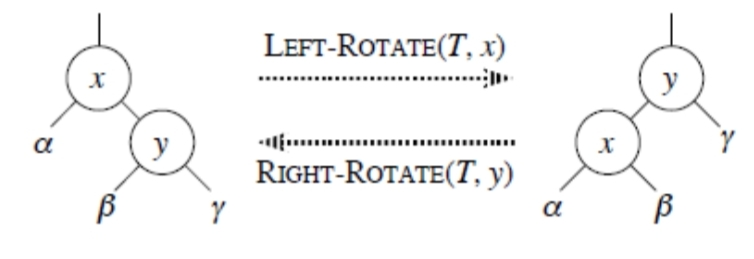
\includegraphics[width=1cm \linewidth]{C:/Users/franc/OneDrive/Desktop/LaTex/Sommario ASD/Immagini/SmartSelect_20231205_160709_Samsung Notes}
%		\end{figure}
%TODO SISTEMA


Lo pseudocodice è:
		\begin{code}{LeftRotate(T,x)}
\li $y \gets \attrib{x}{right}$ \COMMENT{assegna y, nodo che verrà ruotato insieme ad x}
\li $\attrib{x}{h}\gets \proc{MAX(\attribb{x}{left}{h},\attribb{x}{right}{h})}+1$
\li \IF{y.left \neq \attrib{T}{\const{nil}}}
	\li $\attribb{y}{left}{p}\gets x$ \COMMENT{collega} %TODO CONTINUA
		\end{code}
	\end{myParagraph}
\end{formulario}
\end{document}